\graphicspath{{chapters/01_abstract/images}}
\chapter*{Abstract}
\addcontentsline{toc}{chapter}{Abstract}

% The Abstract is a short summary, usually about 1 page in length, that provides the context and the objectives of the project, and summarizes the scientific problem, the techniques used and the results obtained. In case of collaborative work, here is where the graduating student gives details on his or her contribution to the study. Full document should have a maximum of 85 pages, excluding reference list and any appendices.

% TODO: Create graphical abstract
\begin{figure}[!h]
  \centering
  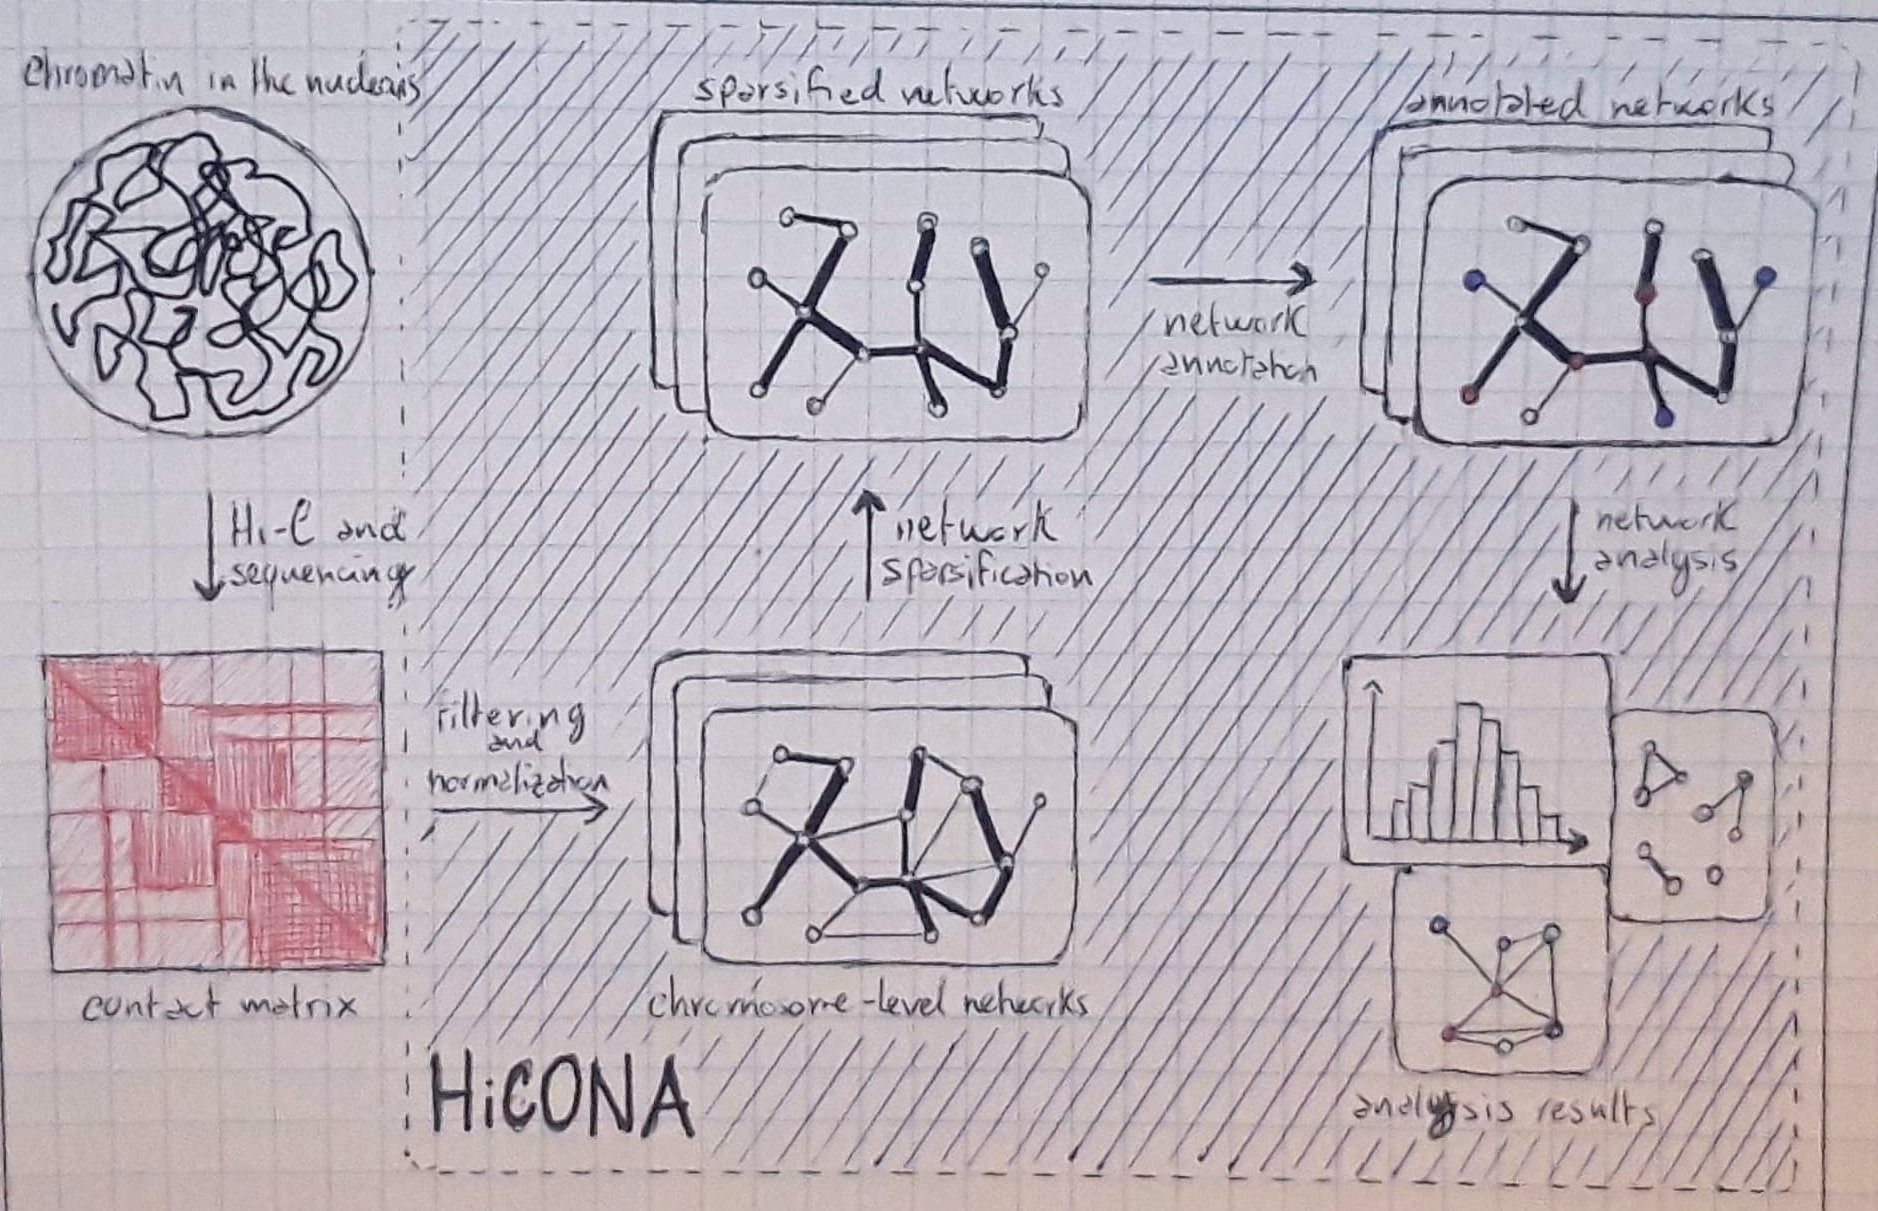
\includegraphics[width=0.80\textwidth]{graphical_abstract.jpeg}
\end{figure}

The usage of network analysis to study chromatin organization is still at a budding state; while there are some tools or some analyses which have been conducted using network analysis algorithms, these tools are generally restricted to a very narrow set of capabilities and can hardly ever be used for analyses different from the main one for which they were designed. Still, network analysis could provide major insights and novel information for this field; for this reason I have been working at the design and implementation of HiCONA, a python3 package aimed at providing a flexible framework in order to conduct any type of network analysis on data coming from Hi-C experiments (a chromosome conformation capture method). The package provides functionalities to create the graph objects, as well as analysis algorithms from both standard network analysis and custom made ones specifically targeted to Hi-C data derived networks. In this thesis the main focus will be on the preprocessing part of the package, how it was implemented, how it works, its performance and comparison with other tools found in literature. Some network analysis will also be discussed, though in a less exhaustive since it is still currently being developed.
